% !TeX program = xelatex
% !TeX encoding = UTF-8
\documentclass[12pt,a4paper]{article}
\usepackage{fontspec}
\usepackage[top=2.54cm,bottom=5.7cm,left=3.18cm,right=3.18cm,headheight=0pt,headsep=0pt,footskip=4.66cm]{geometry}
\setmainfont{NotoSerifSC-Regular.ttf}[Path=build-fonts/,BoldFont=NotoSerifSC-Bold.ttf]
\newfontfamily\headingfont{NotoSansSC-Regular.ttf}[Path=build-fonts/]
\newcommand{\songti}{\normalfont}
\newcommand{\heiti}{\headingfont}
\XeTeXlinebreaklocale "zh"
\XeTeXlinebreakskip=0pt plus 1pt
\usepackage{amsmath,amssymb,mathtools,bm}
\renewcommand{\theequation}{\arabic{equation}}
\usepackage{graphicx}
\usepackage{longtable,booktabs,array,tabularx,calc}
\usepackage{etoolbox}
\usepackage{float}
\usepackage{needspace}
\usepackage{caption}
\usepackage{setspace}
\usepackage{fancyhdr}
\usepackage{titlesec}
\usepackage{tocloft}
\usepackage{indentfirst}
\usepackage{enumitem}
\usepackage{fvextra}
\usepackage{xcolor}
\usepackage{xurl}
\usepackage[hidelinks]{hyperref}
\usepackage{bookmark}
\usepackage{eso-pic}
\usepackage{tikz}
\usetikzlibrary{positioning,arrows.meta,shapes.geometric,fit,backgrounds,calc}
\newcommand{\R}{\mathbb{R}}
\newcommand{\Bset}{\{0,1\}}
\DeclareMathOperator*{\argmin}{arg\,min}
\definecolor{paperGreen}{RGB}{132,168,60}
\definecolor{paperGreenDark}{RGB}{79,96,48}
\definecolor{paperGreenLight}{RGB}{212,224,192}
\definecolor{paperCream}{RGB}{245,243,232}
\tikzset{
  startstop/.style={rectangle,rounded corners=8pt,minimum width=3.2cm,minimum height=0.9cm,align=center,draw=paperGreenDark,fill=paperGreen,text=white,thick},
  process/.style={rectangle,minimum width=3.6cm,minimum height=0.9cm,align=center,draw=paperGreenDark,fill=paperCream,thick},
  decision/.style={diamond,aspect=2.1,minimum width=3.0cm,align=center,draw=paperGreenDark,fill=paperGreenLight,thick,inner sep=1pt},
  data/.style={trapezium,trapezium left angle=70,trapezium right angle=110,minimum width=3.2cm,minimum height=0.9cm,align=center,draw=paperGreenDark,fill=paperGreenLight!55,thick},
  verify/.style={rectangle,minimum width=3.4cm,minimum height=0.9cm,align=center,draw=paperGreenDark,fill=paperGreenLight,thick},
  layer/.style={rectangle,draw=paperGreenDark,dashed,inner sep=6pt},
  arrow/.style={-{Stealth[length=2.4mm]},thick,draw=paperGreenDark},
  lab/.style={font=\small,midway}
}
\newcommand{\sanhao}{\fontsize{16pt}{16pt}\selectfont}
\newcommand{\xiaosan}{\fontsize{15pt}{18.75pt}\selectfont}
\newcommand{\sihao}{\fontsize{14pt}{14pt}\selectfont}
\newcommand{\xiaosi}{\fontsize{12pt}{12pt}\selectfont}
\newcommand{\wuhao}{\fontsize{10.5pt}{10.5pt}\selectfont}
% 正文参考文献编号采用右上角标注
\newcommand{\supcite}[1]{\textsuperscript{[#1]}}

\AtBeginDocument{%
  \xiaosi\songti\setstretch{1.25}%
  % 统一所有行间公式与上下正文之间的距离
  \setlength{\abovedisplayskip}{7.5pt}%
  \setlength{\belowdisplayskip}{7.5pt}%
  \setlength{\abovedisplayshortskip}{7.5pt}%
  \setlength{\belowdisplayshortskip}{7.5pt}%
}
\setstretch{1.25}
\setlength{\parindent}{2em}
\setlength{\parskip}{7.5pt}
\pagestyle{fancy}
\fancyhf{}
\fancyfoot[C]{\xiaosi\thepage}
\renewcommand{\headrulewidth}{0pt}
\renewcommand{\footrulewidth}{0pt}
\fancypagestyle{plain}{\fancyhf{}\fancyfoot[C]{\xiaosi\thepage}\renewcommand{\headrulewidth}{0pt}\renewcommand{\footrulewidth}{0pt}}
\newcommand{\ChineseNumber}[1]{%
  \ifcase#1 零\or 一\or 二\or 三\or 四\or 五\or 六\or 七\or 八\or 九\or 十%
  \or 十一\or 十二\or 十三\or 十四\or 十五\or 十六\or 十七\or 十八\or 十九\or 二十\else #1\fi}
\renewcommand{\thesection}{\ChineseNumber{\value{section}}、}
\renewcommand{\thesubsection}{（\ChineseNumber{\value{subsection}}）}
\renewcommand{\thesubsubsection}{（\arabic{subsubsection}）}
\renewcommand{\theparagraph}{（\arabic{paragraph}）}
\renewcommand{\thesubparagraph}{\arabic{subparagraph}）}
\titleformat{\section}{\centering\heiti\xiaosan}{\thesection}{0.5em}{}
\titlespacing*{\section}{0pt}{12pt}{6pt}
\titleformat{\subsection}{\raggedright\heiti\sihao}{\thesubsection}{0.5em}{}
\titlespacing*{\subsection}{0pt}{6pt}{0pt}
\titleformat{\subsubsection}{\raggedright\songti\xiaosi\bfseries}{\thesubsubsection}{0.5em}{}
\titlespacing*{\subsubsection}{0pt}{6pt}{0pt}
\titleformat{\paragraph}[runin]{\raggedright\songti\xiaosi}{\theparagraph}{0.5em}{}
\titleformat{\subparagraph}[runin]{\raggedright\songti\xiaosi}{\thesubparagraph}{0.5em}{}
\setcounter{secnumdepth}{5}
\setcounter{tocdepth}{3}
% 目录按标题层级逐级缩进：一级顶格，二级和三级依次右移
\cftsetindents{section}{0em}{4em}
\cftsetindents{subsection}{0em}{4em}
\cftsetindents{subsubsection}{0em}{4em}
\makeatletter
\let\paper@l@subsection\l@subsection
\let\paper@l@subsubsection\l@subsubsection
\renewcommand*{\l@subsection}[2]{\paper@l@subsection{\hspace*{2em}#1}{#2}}
\renewcommand*{\l@subsubsection}[2]{\paper@l@subsubsection{\hspace*{4em}#1}{#2}}
\makeatother
\renewcommand{\figurename}{图}
\renewcommand{\tablename}{表}
\DeclareCaptionFont{captioncn}{\songti\xiaosi\setstretch{1.0}}
\DeclareCaptionLabelSeparator{twospaces}{\hspace{2em}}
\captionsetup{font=captioncn,labelsep=twospaces,justification=centering,singlelinecheck=true}
\captionsetup[table]{position=top}
\captionsetup[figure]{position=bottom}
\renewcommand{\thefootnote}{\textcircled{\scriptsize\arabic{footnote}}}
\graphicspath{{media/}}
\makeatletter
\def\maxwidth{\ifdim\Gin@nat@width>\linewidth\linewidth\else\Gin@nat@width\fi}
\def\maxheight{\ifdim\Gin@nat@height>0.82\textheight 0.82\textheight\else\Gin@nat@height\fi}
\def\fps@figure{htbp}
\patchcmd\longtable{\par}{\if@noskipsec\mbox{}\fi\par}{}{}
\makeatother
\AtBeginEnvironment{tabular}{\songti\xiaosi\setstretch{1.0}}
\AtBeginEnvironment{longtable}{\songti\xiaosi\setstretch{1.0}}
\setkeys{Gin}{width=\maxwidth,height=\maxheight,keepaspectratio}
\setlength{\emergencystretch}{3em}
\renewcommand{\arraystretch}{1.15}
\providecommand{\tightlist}{\setlength{\itemsep}{0pt}\setlength{\parskip}{0pt}}
\urlstyle{same}
\hypersetup{pdfauthor={},pdftitle={暖城向新·热力不息}}

\newcommand{\EnableBodyBackground}{%
  \AddToShipoutPictureBG{%
    \AtPageLowerLeft{%
      
\includegraphics[width=\paperwidth,height=\paperheight]{body-background.jpg}%
    }%
  }%
}

\newenvironment{refsectionflush}
  {\par\sloppy\setlength{\parindent}{0pt}\setlength{\parskip}{0pt}}
  {\par\fussy}
\newcommand{\refentry}[2]{%
  \par\noindent\hangindent=2em\hangafter=1
  [#1]\enspace #2\par}

\pretocmd{\section}{\clearpage}{}{}
\widowpenalty=10000\clubpenalty=10000
\begin{document}

\AddToShipoutPictureBG*{%
  \AtPageLowerLeft{
\includegraphics[width=\paperwidth,height=\paperheight]{cover.jpg}}%
}
\thispagestyle{empty}
\null
\clearpage
\EnableBodyBackground
\pagestyle{empty}
\begin{center}
{\songti\sanhao\bfseries\setstretch{1.0} 暖城向新·热力不息\par}
\vspace{18pt}
{\heiti\sihao 摘\quad 要\par}
\end{center}
\vspace{3pt}
\par\indent 面向供热资源、设备、建筑与配电的协同规划，本文以乌鲁木齐、固原和武汉为背景，建立源—网—荷—储与建筑热状态统一约束模型。共享余热预算防止资源重复利用，精确离散1R1C状态连接用户热惯性与区域配电；算法结合硬能量约束的代表日分布校正、费用—碳扫描、连续运行核验及有限管网模式反馈。

六栋外部计量建筑的分布误差中位数由12.3150\%降至4.4775\%，完整准入由3/6提高到4/6。厂家165对Q/P工况支持的三城六组固定资产调度，在共同2880小时内较温控策略降费1.1013\%--1.5970\%。双建筑对照中，配电上限将四倍热容的降费幅度由7.2185\%约束至4.6597\%；72小时网络反馈在第三轮满足水力及远端供温阈值。

研究以公开数据与公共原型开展同条件对照。三城中点碳帽保留80.92\%--89.44\%的降费空间，条件投资给出候选切换预算阈值，费用、物理量及求解界共同支持可解释的方案选择。

\vspace{-4.5pt}
\noindent{\heiti\xiaosi 关键词：}{\songti\xiaosi 源网荷储；建筑热惯性；多目标规划；代表日校正；物理反馈}
\clearpage
\thispagestyle{empty}
\begin{center}{\heiti\sihao 目\quad 录}\end{center}
\begingroup
\fontsize{10.5pt}{12pt}\selectfont\setstretch{1.0}
\setlength{\parskip}{0pt}
\setlength{\cftbeforesecskip}{1pt}
\makeatletter
\@starttoc{toc}
\makeatother
\endgroup
\clearpage
\pagenumbering{arabic}
\setcounter{page}{1}
\pagestyle{fancy}
% !TeX root = ../main.tex
% !TeX program = xelatex
% !TeX encoding = UTF-8
\section{研究问题与技术贡献}

供热转型同时涉及能源替代、既有设施、用热舒适和电网接入。工业余热受到温位和输配约束，分散取暖取决于低温设备能力，夏热冬冷地区需要统筹冷热服务。规划因而必须同时回答资源如何分配、建筑何时用热，以及调度能否满足设备和网络边界。

依据比赛对模型、逐时仿真、多目标、多尺度及代码的要求\supcite{1}，本文以乌鲁木齐、固原和武汉为背景，围绕“物理一致的方案生成—多目标选择—逐时及工程校核”组织研究，并以公共数据对照实验检验方法。

本文的特色集中在四个方面。第一，将共享余热、独立储热和建筑热惯性接入同一能量与状态约束体系，显式限制同一资源的重复分配，并通过区域公用电上限连接建筑调度。第二，将实测负荷的分布保真与能量守恒共同用于代表日权重校正，配合峰值、爬坡和守恒门槛判断压缩方案能否采用。第三，在固定设备研究中使用厂家制热量与输入功率的有效性能域，在网络研究中以校核失败模式的排除推动重新优化，使方案选择响应设备和输配边界。第四，将费用、能量、碳排与求解界分别留痕，给出可核查的条件收益及其代价。

上述贡献体现为模型集成、约束实现与对照实验：以既有热网络、RC及规划方法为基础，通过统一接口连接，并分别验证其作用。

\section{数据基础与三城实验设计}
\subsection{数据来源和用途}

数据按气象驱动、建筑原型、实测计量、设备性能和费用因子分层组织。各层通过对象标识、时间戳与单位映射连接，保留原始文件及变换记录，使模型参数与结果可逐项追溯。表\ref{tab:data-scope}给出数据分工。

\begin{table}[htbp]
\centering
\caption{研究数据及其用途}\label{tab:data-scope}
\begin{tabularx}{\textwidth}{@{}>{\raggedright\arraybackslash}p{0.23\textwidth}X >{\raggedright\arraybackslash}p{0.23\textwidth}@{}}
\toprule
数据依据 & 在本文中的作用 & 证据性质\\
\midrule
NASA POWER逐时气象\supcite{9} & 三城相同窗口下的气候输入；登记时钟、单位及转换 & 公开格点产品\\
BESTEST 600原型\supcite{11} & 建筑几何和热工基准的来源；按登记方法派生1R1C参数 & 公共原型的模型变换\\
BDG2建筑计量\supcite{10} & 六栋建筑的负荷压缩与代表日权重对照 & 外部计量基准\\
TICA产品样本\supcite{12} & 两型号共165个制热量/功率点及缺测角点 & 厂家公开工况表\\
电价及排放因子\supcite{13,14} & 统一比较费用和参考碳排；保留适用条件 & 共同条件性核算\\
OSM空间数据 & 三城建筑与道路候选的空间参考 & 公开空间数据\\
\bottomrule
\end{tabularx}
\end{table}

三城气候对照采用北京时间2024年11月16日00:00至2025年3月16日00:00的左闭右开窗口，共120日、2880个连续小时。建筑与服务条件保持一致，以识别气象影响。费用比较统一采用湖北条件性工商业电价及固定平均排放因子，碳排为同一平均因子下的参考核算。厂家热泵算例将48~m$^2$公共原型合成放大20倍至960~m$^2$，温度边界为20--27~$^\circ$C，初末状态均为20~$^\circ$C。

本文采用两层验证：三城公共原型实验检验同条件调度机制，外部计量实验检验负荷压缩质量。所用连续窗口、资产与边界均随实验登记。

\subsection{三类场景与验证分工}

乌鲁木齐对应既有集中供热与工业余热接入问题，重点是资源共享、温位适配和远端输配；固原对应清洁取暖替代，重点是设备低温能力与接入约束；武汉对应冷热需求与新建系统，重点是建筑热惯性和区域协同。三城均参与统一气候窗口和设备调度对照；网络反馈采用登记的72小时参考系统，公用电耦合采用武汉气象下的双建筑算例。各组实验分别识别气候、设备、建筑柔性和输配约束的作用。

负荷压缩采用BDG2境外建筑计量作为外部基准。三城OSM空间数据承担建筑定位与候选路径表达，资源池通过对象标识关联热源能力和服务对象，实现空间信息与能量约束的分工。

\subsection{统一比较与计量规则}

同一对照固定天气、资产、服务温度、初末状态和计费条件，仅改变所研究的参数或约束。功率、能量、费用与排放分别用kW、kWh、元与kg计量。代表日权重用于汇总，连续状态在原时序中检验；时间轴检查器审核年份、时区和小时连续性。每个结果保存配置、输入指纹、求解状态及独立账本，保证比较可复核。

% !TeX root = ../main.tex
% !TeX program = xelatex
% !TeX encoding = UTF-8
\section{源—网—荷—储与建筑热状态的统一模型}

模型以资源可用量为输入，以建筑交付热量和室内温度为服务输出，将设备转换、区域输配、储热状态及共享电力接入连接为同一约束系统。其优势在于保留能量的物理身份：资源端取热、设备供热、用户交付热量和压缩机用电分别核算，容量投资与逐时调度共同决定可行性。以下功率采用kW，热量采用kWh，温度采用$^\circ$C，温差采用K；时间步长$\Delta t$采用h，连续案例取$1~\mathrm h$。

\begin{figure}[htbp]
\centering
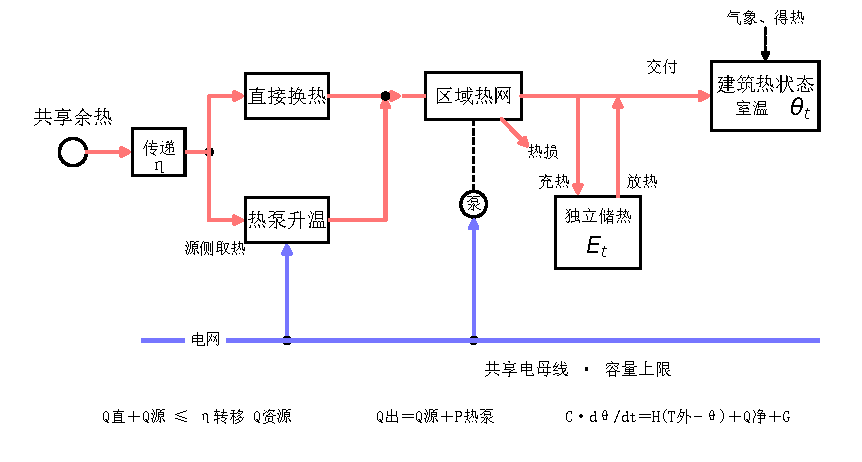
\includegraphics[width=\linewidth]{paper_r2/model_paper/source_network_load_storage_zh.pdf}
\caption{共享资源、热电网络与两类状态的统一结构。热泵源侧取热与电功分别计量；独立储热$E_t$与建筑室温$\theta_t$分别递推。各实验按配置启用模块。}
\label{fig:unified-structure}
\end{figure}

\subsection{资产容量与共享热资源}

令$k,n,g,b,s,e,t$分别表示设备、区域节点、供热温位、建筑、储热装置、管段和时段。源设备的现有、新增与退役容量共同约束各温位出力：
\begin{equation}
K_k=K_k^{\mathrm{exist}}+K_k^{\mathrm{new}}-K_k^{\mathrm{ret}},
\qquad
0\leq\sum_g Q_{k,g,t}\leq a_{k,t}K_k .
\label{eq:scoring-capacity}
\end{equation}
其中$a_{k,t}$为逐时可用率；新增上限、政策退役、启停、最小出力及爬坡由对应设备配置加载。容量约束按同一设备聚合出力，避免将不同温位视作互不占用容量的独立热源。

同一余热或可再生资源可同时连接直接换热设备与热泵，因而还需约束资源池$r$的共同取用量：
\begin{equation}
R_{r,t}^{\mathrm{use}}
=\frac{1}{\eta_r^{\mathrm{tr}}}
\left[
\sum_{k\in\mathcal D_r,g}Q_{k,g,t}
+\sum_{k\in\mathcal H_r,g}
\left(1-\frac{1}{\mathrm{COP}_{k,g,t}}\right)Q_{k,g,t}
\right]
\leq \overline R_{r,t}.
\label{eq:scoring-resource}
\end{equation}
$\eta_r^{\mathrm{tr}}\in(0,1]$为资源端至设备端的传热效率，$\mathcal D_r$与$\mathcal H_r$分别为直接换热和热泵成员。直接换热按交付量折算上游需求；热泵先扣除压缩机电功，再折算资源取热。两种路径因而共同占用同一个逐时资源预算，防止同一份余热被重复利用。资源池与成员唯一关联，资源传热、设备转换及管网输送分别核算，使瓶颈可定位到具体环节。

\subsection{设备性能域与温位适配}

通用模型以外生逐时$\mathrm{COP}$、$\mathrm{EER}$及效率描述转换，热泵与电锅炉分别满足
\begin{equation}
Q^{\mathrm{HP}}=\mathrm{COP}\,P^{\mathrm{HP}},\qquad
Q^{\mathrm{EB}}=\eta^{\mathrm{EB}}P^{\mathrm{EB}} .
\label{eq:scoring-conversion}
\end{equation}
直接热源仅接入其供水温度能够满足的温位；热泵按提升后的供热侧温位交付。温位由此同时影响资源取热、耗电与可连接用户。

厂家性能域算例进一步保留同型号、同工况的成对供热量$Q^{\mathrm{cat}}$与输入功率$P^{\mathrm{cat}}$。对相邻打印坐标分别插值，而后计算比值：
\begin{equation}
\begin{aligned}
Q_t^{\mathrm{cat}}&=\sum_i\lambda_{i,t}Q_i,\qquad
P_t^{\mathrm{cat}}=\sum_i\lambda_{i,t}P_i,\\
\mathrm{COP}_t^{\mathrm{cat}}&=\frac{Q_t^{\mathrm{cat}}}{P_t^{\mathrm{cat}}},\qquad
\lambda_{i,t}\geq0,\quad \sum_i\lambda_{i,t}=1 .
\end{aligned}
\label{eq:scoring-performance}
\end{equation}
权重由外生环境温度和出水温度的相邻坐标确定，作为预计算系数进入优化；有效域同时检查插值角点。在准入时段，固定整机算例采用声明的交付能力系数$\phi\in(0,1]$：
\begin{equation}
0\leq Q_t^{\mathrm{HP}}\leq\phi Q_t^{\mathrm{cat}},\qquad
P_t^{\mathrm{HP}}=
\frac{P_t^{\mathrm{cat}}}{\phi Q_t^{\mathrm{cat}}}Q_t^{\mathrm{HP}} .
\label{eq:scoring-duty}
\end{equation}
成对Q/P将工况变化同时传递至出力上限与单位供热耗电，使设备能力和配电占用采用一致依据。该式以理想小时占空比描述部分负荷运行，厂家表的型号、单位和工况随性能记录保存。

\subsection{节点守恒与网络物理反馈}

零失供服务下，各节点按温位逐时守恒：
\begin{multline}
\sum_{k\in\mathcal K_n}Q_{k,g,t}
+\sum_{e\in\delta^-(n)}\eta_{e,t}F_{e,g,t}
+\sum_{s\in\mathcal S_{n,g}}Q_{s,t}^{\mathrm{dis}}\\
=D_{n,g,t}+\sum_{b\in\mathcal B_{n,g}}Q_{b,t}^{\mathrm h}
+\sum_{s\in\mathcal S_{n,g}}Q_{s,t}^{\mathrm{ch}}
+\sum_{e\in\delta^+(n)}F_{e,g,t}.
\label{eq:scoring-node}
\end{multline}
$F$为管段入口功率，$\eta_{e,t}$为交付效率，故$(1-\eta_{e,t})F$为损失。$D$只表示未被建筑热状态模块覆盖、并已计入启用需求侧调整的有效固定服务，已覆盖部分以实际建筑交付量替代原负荷列。双向管段按实际方向计入，候选容量与改造状态限制输送，循环泵电耗同步进入电力账本。

有限模式网络接口将给定流量、回水温度下的双管散热、水力阻力及泵效率换算为交付效率和泵功率：
\begin{equation}
\eta_m^{\mathrm{net}}=\frac{Q_m^{\mathrm{out}}}{Q_m^{\mathrm{in}}},
\qquad
P_m^{\mathrm{pump}}=
\frac{\Delta p_m\dot m_m}{1000\,\rho\,\eta_m^{\mathrm{pump}}}.
\label{eq:scoring-network}
\end{equation}
其中压差采用Pa，质量流量采用kg/s，密度采用kg/m$^3$。求解后按运行模式的瞬时状态校核远端温度、流速、压降和泵功率；不合格模式被切除后重新求解，并保留每轮记录。这使热量平衡与工程可行性形成可追踪的反馈。

\subsection{建筑热状态与精确逐时递推}

建筑采用单状态1R1C结构\supcite{2}，将围护与换气损失、建筑蓄热及内外得热显式纳入服务约束：
\begin{align}
C_b\frac{\mathrm d\theta_b}{\mathrm dt}
&=H_b(T^{\mathrm{out}}-\theta_b)+Q_b^{\mathrm h}-Q_b^{\mathrm c}+G_b,
\label{eq:scoring-rc-cont}\\
a_b&=\exp(-H_b\Delta t/C_b),\qquad
\beta_b=(1-a_b)/H_b,\\
\theta_{b,t}
&=a_b\theta_{b,t-1}+(1-a_b)T_t^{\mathrm{out}}
+\beta_b(Q_{b,t}^{\mathrm h}-Q_{b,t}^{\mathrm c}+G_{b,t}).
\label{eq:scoring-rc}
\end{align}
$H_b$采用kW/K，$C_b$采用kWh/K，$G_b$为内部与太阳得热之和，采用kW。式\eqref{eq:scoring-rc}是区间输入保持下的精确积分，温度变量表示时段末状态；实现采用稳定指数差计算，避免小时间步下的相消误差。

逐时温度上下界直接约束状态，供热与供冷采用有限功率上界，启用互斥时以二元变量排除同楼同时冷热供给。交付功率既驱动状态，又进入式\eqref{eq:scoring-node}，预热必须占用设备及配电能力。各连续组由声明初温递推至规定终温或区间，不再叠加虚拟储热需求。同服务比较固定舒适和初末状态，以排除透支终端蓄热的收益；逐楼状态与交付量均导出复算。

\subsection{独立储热的连续性与边界}

储热与建筑状态分别建模。以下$t=1,\ldots,T$，$E_{s,0}$是首小时开始前状态。令$K_s^E$为现有与新增能量容量，$r_s$为功率能量比，单位h$^{-1}$，则
\begin{align}
E_{s,t}
&=(1-\mu_s)^{\Delta t}E_{s,t-1}
+\eta_s^{\mathrm{ch}}Q_{s,t}^{\mathrm{ch}}\Delta t
-Q_{s,t}^{\mathrm{dis}}\Delta t/\eta_s^{\mathrm{dis}},
\label{eq:scoring-storage}\\
0\leq E_{s,t}&\leq K_s^E,\qquad
0\leq Q_{s,t}^{\mathrm{ch}},Q_{s,t}^{\mathrm{dis}}\leq r_sK_s^E .
\end{align}
$\mu_s$为每小时自损失率，充、放热效率均为无量纲；严格模式以二元变量约束充放互斥。固定初态采用$E_{s,0}=f_s^{\mathrm{init}}K_s^E$，组末要求$E_{s,\mathrm{end}}\geq f_s^{\mathrm{final}}K_s^E$；循环边界连接组首与组末。容量、充放功率及温位分别限定移峰深度、持续时间与服务对象。组内状态连续递推，代表期权重仅累计费用和能量。安装容量及边界随案例登记；建筑RC及多尺度案例采用空储热集以识别建筑自身的柔性。

\subsection{共享电力与多尺度耦合}

各电驱热源、制冷设备及循环泵的功率合并为系统电负荷：
\begin{align}
P_t^{\mathrm{sys}}
&=\sum_{k,g}\frac{Q_{k,g,t}^{\mathrm{HP}}}{\mathrm{COP}_{k,g,t}}
+\sum_k\frac{Q_{k,t}^{\mathrm{EB}}}{\eta_k^{\mathrm{EB}}}
\notag\\
&\quad+\sum_k\frac{Q_{k,t}^{\mathrm c}}{\mathrm{EER}_{k,t}}
+\sum_eP_{e,t}^{\mathrm{pump}},
\notag\\
(1+\sigma)P_t^{\mathrm{sys}}&\leq a_t^{\mathrm{grid}}K^{\mathrm{grid}}.
\label{eq:scoring-electric}
\end{align}
该式对应无微电网的共享接入约束，$\sigma$为备用裕度。启用微电网时，充电增加进口需求，本地发电与放电减少进口需求，并约束进口非负。统一电负荷注册表同时服务配电约束和电量统计，重复注册或冻结后漏加负荷会直接报错。系统接入投资传递至区域设备运行，节点聚合再传递至逐楼交付与温度状态；共享上限绑定时，各建筑通过真实电力竞争发生耦合。

\subsection{经济与系统碳的共同账本}

费用和碳排采用相同物理调度量及时间权重。设$\omega_t=\pi_t w_t\Delta t$，其中$\pi_t$为情景概率、$w_t$为代表期频数权重，基本账本为
\begin{equation}
\begin{aligned}
C_0={}&\mathrm{CRF}\,I_{\mathrm{net}}+C_{\mathrm{fix}}+C_{\mathrm{event}}+C_{\mathrm{basic}}+C_{\mathrm{other}}
+\sum_t\omega_t\,\boldsymbol c_t^\mathsf T\boldsymbol x_t,\\
\mathcal E={}&\mathcal E_{\mathrm{const}}+\sum_t\omega_t\,\boldsymbol e_t^\mathsf T\boldsymbol x_t .
\end{aligned}
\label{eq:scoring-ledger}
\end{equation}
$\boldsymbol x_t$为逐时运行变量向量；费用以元、碳排以kg计。$C_{\mathrm{event}}$、$C_{\mathrm{basic}}$和$C_{\mathrm{other}}$分别汇总启停、基本电费及其他启用费用。后文采用$F_C=C_0+C_{\mathrm{carbon}}+C_{\mathrm{pref}}$、$F_E=\mathcal E$。投资扣除声明补贴后年化，设备、泵及本地供电按共同调度量计费；供热、供冷和共享电力合计碳排后施加碳帽，使经济与环境目标比较同一份服务。

地源设备逐源、逐情景累计供热取热与供冷排热，分别扣除与计入压缩机电耗；启用年度比例时检查
\begin{equation}
r_j^{\min}E_j^{\mathrm{rej}}\leq E_j^{\mathrm{ext}}
\leq r_j^{\max}E_j^{\mathrm{rej}} .
\label{eq:ground-ledger}
\end{equation}
以上约束通过统一变量与节点接口装配。网络、储热和地源模块按场景配置启用，形成面向不同服务边界的可复用模型。

% !TeX root = ../main.tex
% !TeX program = xelatex
% !TeX encoding = UTF-8
\section{多目标规划与物理反馈求解}

\subsection{费用与系统碳的容差端点及约束扫描}

技术、管网和运行模式选择含整数变量，能流、容量与热状态为连续变量，装配后形成有限规模MILP。费用目标为
\begin{equation}
F_C=C_0+C_{\mathrm{carbon}}+C_{\mathrm{pref}},\qquad F_E=\boldsymbol a_E^\mathsf T\boldsymbol x+E_0,
\label{eq:scoring-objectives}
\end{equation}
其中偏好与惩罚单列，系统碳采用冷热服务及共享电力的一致台账，常数项$E_0$保留。所有方案沿用相同的可靠性、舒适、设备和资源硬边界，防止通过减少服务获得虚假减碳。

为处理单目标的同值替代解，先以费用为主、系统碳为次求一个端点，再交换次序、新建模型求另一端点\supcite{5}。第一阶段获得主目标可行值$v_1$后，第二阶段加入
\begin{equation}
f_1\leq v_1+\delta_{\mathrm{abs}}+\delta_{\mathrm{rel}}|v_1|,
\qquad\min f_2.
\label{eq:scoring-endpoint}
\end{equation}
接口默认$\delta_{\mathrm{abs}}=10^{-7}$，量纲随主目标，$\delta_{\mathrm{rel}}=10^{-8}$；两阶段分别登记状态、时限、原始界与gap。若第一阶段仅返回限时可行解，第二阶段以该可行值为锚点，其身份仍为容差边界内的次目标改进。

随后在端点碳区间内按登记档位求解$\min F_C$、$F_E\leq\varepsilon_E^{\mathrm{eff}}$，其中$\varepsilon_E^{\mathrm{eff}}=\varepsilon_E+10^{-7}+10^{-8}|\varepsilon_E|$。专用扫描入口将碳价置零，赛事入口保留配置中的碳价与偏好项，两类目标分别标注。每档复核碳帽与数值可行性，对可行样本去重并剔除支配点，形成有限采样下的非支配方案集合。碳帽具有明确物理单位，便于直接回答“给定排放额度下能以多少费用满足服务”。

\subsection{实际日选取与硬能量约束下的权重校正}

代表日首先将同源气象、负荷等逐时特征按日展开、标准化，以K-means聚类，再取各簇距中心最近的实际日。随后保留系统及各服务负荷峰值、最大真实相邻小时爬坡、最低气温和已配置的资源风险日；跨午夜最大爬坡保留两侧日期，新增极值日的频数从原簇扣除，使总日数守恒。

频数权重保证覆盖次数，却可能使压缩后的总能量和负荷持续分布偏离原序列。为此，在固定选日集合上仅校正权重。设保留观测含$D$个完整日，每日$H=24$小时，实际日轮廓为$q_{jh}$，$E_j=\sum_hq_{jh}\Delta t$；在观测与代表值联合支撑点$s_i$上计算经验分布$F_o$及加权分布$F_w$，求解
\begin{equation}
\begin{aligned}
\min_{\boldsymbol w}\;&\frac{1}{\bar q}\sum_i(s_{i+1}-s_i)
       |F_w(s_i)-F_o(s_i)|,\\
\text{s.t.}\;&\sum_jw_j=D,\quad \sum_jw_jE_j=E_o,\quad w_j\geq\ell_j,\\
F_w(s_i)=\;&\frac{1}{HD}\sum_jw_j\sum_{h=1}^{H}\mathbf1(q_{jh}\leq s_i).
\end{aligned}
\label{eq:scoring-hard-w1}
\end{equation}
其中$\bar q>0$，$E_o$为同一保留序列的总能量。绝对值用辅助变量线性化，由HiGHS求解标准LP，并独立重算能量、日数、下界和目标残差。冻结六楼规程对极值日取$\ell_j=1$日，其余取$10^{-6}$日；校正不改原观测或日轮廓。

候选还须通过预先登记的统计准入：相对能量误差不超过0.1\%，同口径归一$W_1$不劣于频数基线，保留序列峰值、真实相邻爬坡及原始观测峰值保留率均达到1。失败时保存原因并回退频数权重，回退方案另行验收。事件覆盖由选日与峰值检查保证，权重校正优化既定样本的分布；状态可行性由连续回放检查。

\subsection{固定投资原时序回放与管网反馈}

规划结果保存技术、容量、管网、储热和接入选择，并通过冻结审计固定全部投资；原时序仅重新调度。回放先核对输入指纹、真实时间戳、容量与服务边界，再连续递推建筑及储热状态，独立复算舒适、能量和初末条件。接口覆盖所给连续窗口，三城共同2880小时窗口及其控制策略试验分别登记。统计压缩承担规划计算，原时序审核承担运行准入。

管网反馈进一步处理线性调度解与瞬时热水输送条件的差异。当前实现限定于独立泵星型支路、定物性水和有限个固定流量、回水温度稳态模式。每个模式计算两程散热、远端供水、摩阻和泵电力。令$z_{mt}$表示模式启用，则
\begin{equation}
0\leq q_{mt}\leq Q_m^{\mathrm{in}}z_{mt},\quad
\sum_{m\in b}z_{mt}\leq1;
\qquad z_{mt}=0\quad(m\in\mathcal B^{(k)},\ \forall t),
\label{eq:scoring-network-cut}
\end{equation}
其中$\mathcal B^{(k)}$为第$k$轮发现的不合格模式。小时平均交付量按占空比计算，但流速、压力、泵功率和供回温边界按启用瞬时值核查；源容量与电力接入亦按同时启用模式约束。每轮重新计算源热、交付热、散热及泵电台账，失败模式全时段禁用后重新求解；无新增有效排除、求解失败或轮数耗尽均停止并留痕。有限目录逐步缩减，因此每次有效反馈至少消去一个模式。温差软惩罚单独核算，其作用须由开关对照确认；当前试验的可行性改善来自硬校核排除。该反馈不涵盖输送时滞、启停瞬态或共泵水力平衡。

\subsection{同目标收敛证据与模块衔接}

核心模型经SciPy的\path{milp}接口调用HiGHS\supcite{6,7}。结果同时保存终止状态、可行解、矩阵及整数残差、目标重算和gap。最小化问题的可行目标值$U$与求解器下界$L$采用相同目标，含常数项时共同加回；限时可行解与容差内最优解分别标注。固定设备热泵LP另以精确有理运算处理已编码binary64系数，形成电量费目标的弱对偶下界。该证书与数值解的可行性容差共同说明解的质量，便于不同边界与时限下复核收敛结果。

模块通过输入身份、服务合同和固定资产记录衔接。多目标端点与碳帽扫描形成取舍集合，$W_1$校正提高输入分布保真，连续回放及物理反馈检查服务可达性。第七章以伪代码展开各入口的调用、停止和复现逻辑。

% !TeX root = ../main.tex
% !TeX program = xelatex
% !TeX encoding = UTF-8
\section{对照实验与机制分析}
\subsection{实测负荷的分布保真与准入}

在六栋外部计量建筑上，固定各自选取的8--10个代表日，仅比较软校正与硬能量约束下的最小Wasserstein距离权重。归一分布误差定义为一阶Wasserstein距离除以同一保留完整日序列的平均负荷。表\ref{tab:w1}列出全部六例，所示中位数仅描述这一组样本。

\begin{figure}[htbp]
\centering
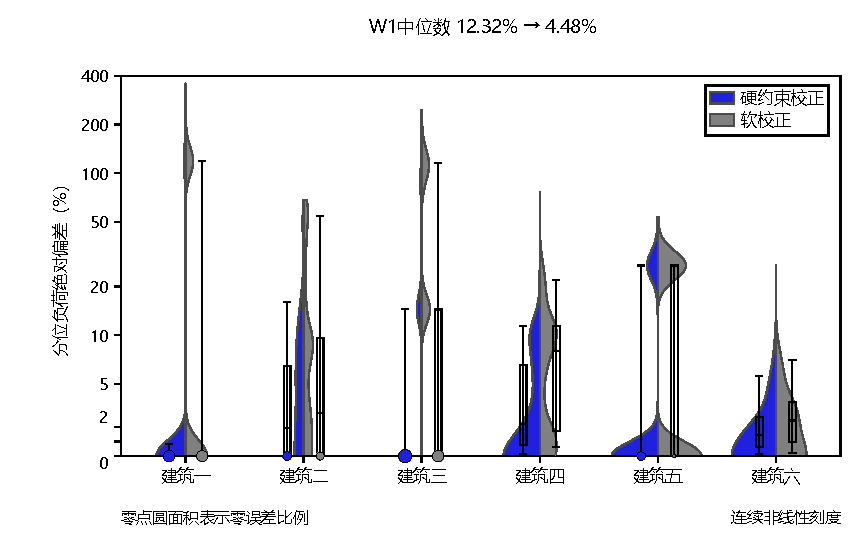
\includegraphics[width=\linewidth]{paper_r2/external_w1.pdf}
\caption{六建筑固定代表日的分布校正。蓝、灰分别表示硬约束与软校正；箱线为加权分位，零点圆面积为零偏差比例。纵轴采用连续非线性刻度，保留完整尾部。}
\label{fig:w1-distribution}
\end{figure}

图\ref{fig:w1-distribution}按相同累计概率匹配原始与代表负荷，绘制归一绝对偏差及其概率分布；箱体为25/50/75分位，须为5/95分位，均由原离散概率质量计算。加权平均偏差等于对应$W_1$，使分布形态与误差指标直接对应；小提琴轮廓仅用于密度展示。

\begin{table}[htbp]
\centering
\caption{固定代表日集合的权重校正结果}\label{tab:w1}
\begin{tabularx}{\textwidth}{@{}lrrX@{}}
\toprule
建筑 & 软校正误差/\% & 硬约束误差/\% & 硬约束候选的完整准入\\
\midrule
一 & 18.0043 & 4.8097 & 通过\\
二 & 10.0363 & 4.9463 & 原始峰值覆盖不足\\
三 & 20.9090 & 4.1453 & 新增通过\\
四 & 8.2519 & 3.8920 & 通过\\
五 & 14.5937 & 5.4303 & 原始峰值覆盖不足\\
六 & 2.7885 & 2.0065 & 通过\\
\midrule
中位数 & 12.3150 & 4.4775 & 通过数量由3/6增至4/6\\
\bottomrule
\end{tabularx}
\end{table}

六例分布误差均下降，说明相同代表日预算下的保真度得到改善。能量、峰值与爬坡门槛同时筛选规划输入，完整统计准入由3/6提高到4/6。该年度内部压缩实验表明，分布校正与极端事件检查能够互补：前者优化权重，后者保证关键负荷得到覆盖。

\subsection{厂家性能域下的固定设备调度}

对TCAV035BHE与TCAV065BHE分别登记83、82个Q/P工况点，并保留15个缺失角点。插值遵守有效单元和型号身份，对缺角、越界或跨型号查询执行拒绝。在每个城市、每个固定型号配置内，比较温控策略与条件电量费最小LP；六组对照均覆盖连续2880小时，设备台数、舒适和末状态保持相同。

\begin{table}[htbp]
\centering
\caption{同资产LP相对温控策略的条件运行收益}\label{tab:heatpump}
\begin{tabularx}{\textwidth}{@{}lXrrr@{}}
\toprule
城市 & 型号 & 降费/\% & 少付费用/元 & 增加电量/kWh\\
\midrule
乌鲁木齐 & TCAV035BHE & 1.3274 & 798.75 & 1398.80\\
乌鲁木齐 & TCAV065BHE & 1.1088 & 474.44 & 753.51\\
固原 & TCAV035BHE & 1.4526 & 908.06 & 1548.64\\
固原 & TCAV065BHE & 1.1013 & 491.80 & 874.83\\
武汉 & TCAV035BHE & 1.1268 & 173.35 & 364.93\\
武汉 & TCAV065BHE & 1.5970 & 237.79 & 728.99\\
\bottomrule
\end{tabularx}
\end{table}

表\ref{tab:heatpump}为固定资产LP数值最优解，求解界按登记编码模型核验。六例通过移时降费1.1013\%--1.5970\%，同时增加电量及固定平均因子碳排，揭示价格激励与能效目标的差异。Q/P有效域保留工况对能力的影响，理想小时占空比刻画可调度空间。

\subsection{热容与区域配电约束的交互}

为独立识别建筑热容效应，保留两个建筑的温度状态。建筑A固定$H=0.1043$~kW/K、$C=0.535576$~kWh/K；建筑B固定$H=0.15645$~kW/K，仅将$C$从0.535576改为2.142304~kWh/K。另一实验轴为是否施加6.4796375~kW的共同用电上限。四案均使用同一武汉气象、2880小时、既有理想设备和20--27~$^\circ$C服务边界。

\begin{table}[htbp]
\centering
\caption{热容倍率与公用电上限的二维对照}\label{tab:factorial}
\begin{tabularx}{\textwidth}{@{}Xrrrr@{}}
\toprule
研究设置 & 电量费/元 & 用电/kWh & 峰值/kW & 绑定小时\\
\midrule
原热容，无公用上限 & 5918.14 & 8155.11 & 14.1064 & ---\\
四倍热容，无公用上限 & 5490.94 & 8725.44 & 25.3335 & ---\\
原热容，有公用上限 & 5937.64 & 8050.61 & 6.4796 & 125\\
四倍热容，有公用上限 & 5660.96 & 8386.07 & 6.4796 & 530\\
\bottomrule
\end{tabularx}
\end{table}

四案均得到求解器容差内最优解，保存的MIP gap为0。共同上限下，增大热容使电量费下降276.68元，即4.6597\%；无共同上限时下降427.20元，即7.2185\%。两者之差150.52元量化了配电约束对热容经济价值的影响。共同上限下，区域用电增加335.46~kWh；独立积分账本将其分解为建筑A热损减少53.94~kWh与建筑B热损增加389.40~kWh，解释预热移时的能量代价。

\begin{figure}[htbp]
\centering
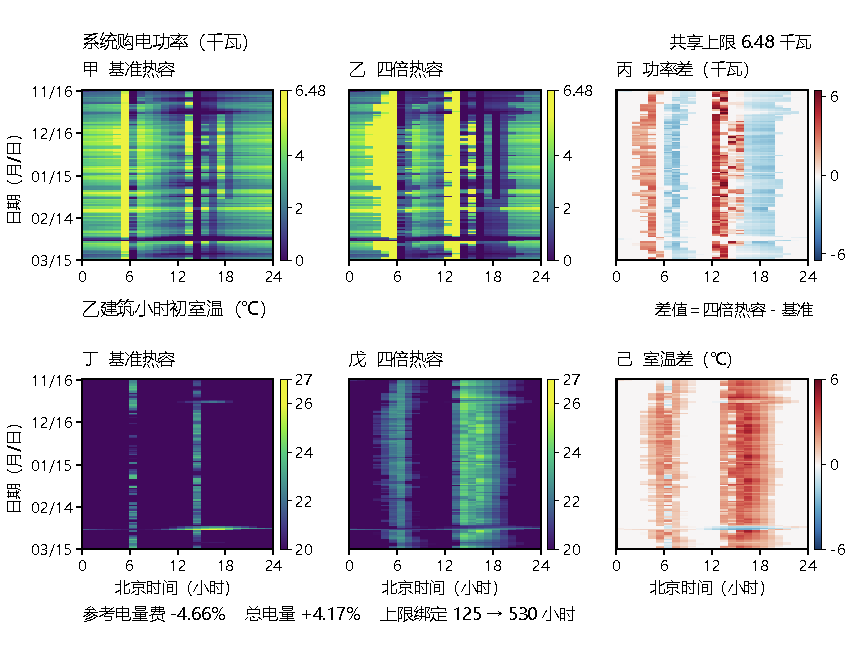
\includegraphics[width=\linewidth]{paper_r2/mechanism_paper/thermal_coupling.pdf}
\caption{共享配电边界下的热惯性调度。上排为系统购电功率，下排为乙建筑小时初室温；第三列为四倍热容减基准。图示完整120日逐时状态，显示预热时移及其容量占用。}
\label{fig:thermal-coupling}
\end{figure}

图\ref{fig:thermal-coupling}将预热与购电时移对应起来：用户热状态通过区域电力上限影响系统费用，热容价值取决于共享约束。该对照识别区域—建筑层的交互，城市级容量选择由规划接口承载。

\subsection{管网校核反馈与可行性成本}

在72小时参考系统上，对优化输出逐支路检查压降梯度、远端供水温度及热量账本。发现不满足阈值的模式后，排除该模式并重新优化。三轮对同一交付热量191.5475~kWh的结果见表\ref{tab:network}。

\begin{table}[htbp]
\centering
\caption{有限网络模式反馈的三轮结果}\label{tab:network}
\begin{tabularx}{\textwidth}{@{}Xrrr@{}}
\toprule
指标 & 第一轮 & 第二轮 & 第三轮\\
\midrule
最大压降梯度/(Pa/m) & 1081.42 & 504.33 & 237.96\\
最低远端供水温度/$^\circ$C & 61.52 & 59.85 & 57.45\\
管路热损/kWh & 35.70 & 56.94 & 94.44\\
泵耗/kWh & 0.7101 & 0.3570 & 0.1901\\
参考费用/元 & 178.64 & 195.01 & 224.26\\
校核结论 & 压降超限 & 压降超限 & 通过\\
\bottomrule
\end{tabularx}
\end{table}

第三轮满足压降梯度不大于300~Pa/m、远端供水不低于55~$^\circ$C的阈值，得到参考运行费用224.26元的可行方案。模式调整降低泵耗与压降，同时增加热损和源需求，对应费用增加25.54\%。失败模式排除与重求解自动完成这一修正，使温压可行性与其费用代价共同进入方案选择。

\subsection{三城费用—碳排取舍}

三城固定理想资产小原型以同一温控反馈策略为基准，求电量费端点、碳端点及中点碳帽。资产与厂家热泵实验不同，表\ref{tab:tradeoff}比较各自基准下的增排与降费取舍。

\begin{table}[htbp]
\centering
\caption{三城中点碳帽方案的决策取舍}\label{tab:tradeoff}
\begin{tabular*}{\textwidth}{@{\extracolsep{\fill}}lrrrr@{}}
\toprule
城市 & 费用端降费/\% & 中点降费/\% & 中点增排/\% & 降费保留/\%\\
\midrule
乌鲁木齐 & 1.7012 & 1.3916 & 1.7716 & 81.80\\
固原 & 1.7168 & 1.3892 & 1.7469 & 80.92\\
武汉 & 1.7518 & 1.5668 & 2.2003 & 89.44\\
\bottomrule
\end{tabular*}
\end{table}

\begin{figure}[htbp]
\centering
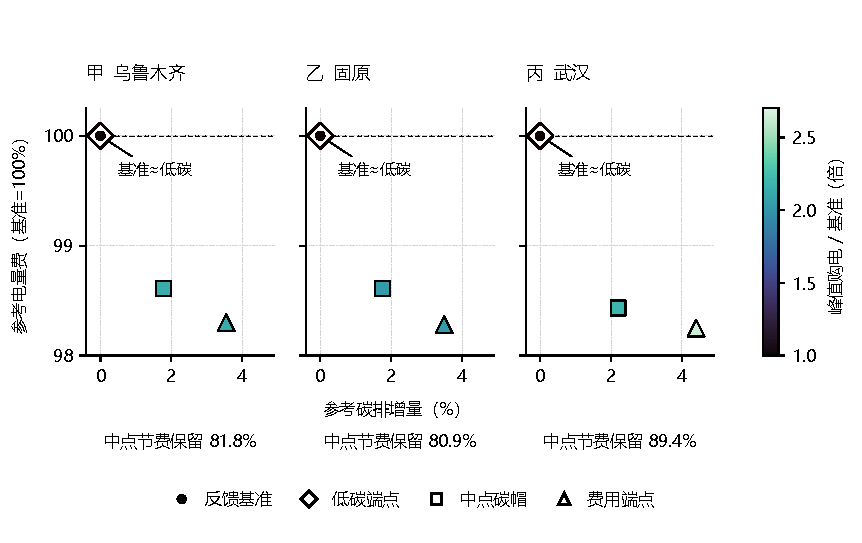
\includegraphics[width=\linewidth]{paper_r2/tradeoff_paper/cost_carbon.pdf}
\caption{三城登记方案的费用、碳排与峰值取舍。图示固定资产实际点，颜色表示峰值与各自基准的比值；中点节费保留率的分母为费用端点相对基准的节省额。}
\label{fig:cost-carbon}
\end{figure}

优化点为固定资产问题的登记容差内最优调度。中点碳帽将电量费端点相对基准的增排约减半，保留80.92\%--89.44\%的降费；对应相对基准增排1.75\%--2.20\%。图\ref{fig:cost-carbon}同步呈现峰值占用，中点为基准的2.04--2.21倍，为联合设置碳帽与配电容量提供依据。

% !TeX root = ../main.tex
% !TeX program = xelatex
% !TeX encoding = UTF-8
\section{经济评价与方案选择}
\subsection{同口径费用与碳排比较}

同资产调度固定天气、服务温度和初末状态，比较费用、能耗、峰值及碳排。表\ref{tab:heatpump}回答既有设备如何优化运行，表\ref{tab:tradeoff}回答排放额度如何改变费用选择；共同调度轨迹给出收益的物理解释。

投资评价将年化或折现账本与运行分析衔接。给定同等服务下的增量投资$\Delta I$、年度能源费用节约$\Delta B_y$、新增维护$\Delta M_y$、更新费用$\Delta R_y$及残值差$\Delta V_Y$，净现值为
\begin{equation}
\mathrm{NPV}=-\Delta I+\sum_{y=1}^{Y}\frac{\Delta B_y-\Delta M_y-\Delta R_y}{(1+r)^y}+\frac{\Delta V_Y}{(1+r)^Y},
\label{eq:npv}
\end{equation}
其中$r$为折现率。本式给出项目现金流的统一接口；以下条件投资实验采用独立登记的采购预算和重复窗口账本，以价格阈值说明候选方案的选择机制。

\subsection{采购价格阈值与方案敏感性}

条件投资实验登记0、1、2台热泵候选，在相同2880小时服务与固定性能假设下求解五档碳帽，得到三个不同方案。比较账本为采购预算加$F=5$个120日重复窗口的能源费用及假设维护预算；$F$是研究设计系数。该实验的设备价格与性能身份独立于前述TICA厂家性能域实验。

令$p\geq0$为每台候选设备的采购预算，固定其他条件后，各台数下的最小比较费用可以写成
\begin{equation}
B_0(p)\approx14402.3788,\quad
B_1(p)\approx p+5055.8954,\quad
B_2(p)\approx2p+5455.8596.
\label{eq:price-lines}
\end{equation}
金额单位均为元，截距来自各固定台数下的运行最优解，展示值经四舍五入。两台方案满足$B_2-B_1\approx p+399.9641>0$；按原值计算，一台方案与零台方案的交点为
\begin{equation}
p^*=B_0(0)-B_1(0)\approx9346.4833\ \text{元}.
\label{eq:price-threshold}
\end{equation}
在$F=5$账本及非负价格域内，$p<p^*$选择一台，$p>p^*$选择零台，交点处费用相同。配套投资增量$\Delta K$及每窗口维护增量$\Delta M$使一台方案的优势条件变为\mbox{$p+\Delta K+5\Delta M\leq p^*$}，由此定位预算变化导致的方案切换。

% !TeX root = ../main.tex
% !TeX program = xelatex
% !TeX encoding = UTF-8
\section{软件组织与可复现性}

工程将输入验证、模型与求解函数置于\path{src/heatplan/}，运行编排置于命令行及\path{scripts/}。场景参数通过配置传入，函数以具名字段返回方案、诊断和状态；注释说明单位、边界及求解身份，同一约束库可复用于不同场景。

以下伪代码对应实际实现。四个算法按各自入口执行，共用输入验证、求解与证据规范。

\subsection{配置分派与结果输出}
\noindent\textbf{算法1：场景清单主程序。}输入：场景清单、配置与时序路径、时限及gap；输出：逐场景方案、比较表和运行参数。
\begin{longtable}{@{}p{0.07\textwidth}p{0.88\textwidth}@{}}
\toprule 行 & 操作\\\midrule
\endfirsthead
\toprule 行 & 操作（续）\\\midrule
\endhead
\bottomrule\endfoot
01 & 读取清单，解析相对路径；校验命令行gap及可选政策配置。\\
02 & \textbf{对每个}场景条目，创建独立输出目录并读取配置路径。\\
03 & \quad\textbf{若}提供阶段路径，\textbf{则}调用阶段规划函数，保存阶段与投资表。\\
04 & \quad\textbf{否则}读取并验证配置及时序；按可选情景定义构造输入并再次验证。\\
05 & \quad\quad{}装配\texttt{HeatPlanningModel}，调用\texttt{solve}，导出方案。\\
06 & \quad{}汇总该场景状态；\textbf{若}配置政策评价，\textbf{则}保存评价表。\\
07 & \textbf{结束循环}；保存场景比较表及实际时限、gap覆盖规则。\\
08 & 输出运行摘要并\textbf{返回}控制台；异常由对应调用报告。\\
\end{longtable}
普通规划输出由\texttt{export\_results}统一生成费用碳摘要、投资、调度及已附加的建筑审核表；冻结研究入口另保存输入及代码指纹、失败文件和manifest，便于反查每个表值的实际运行。

\Needspace{15\baselineskip}
\subsection{硬能量校正、准入与回退}
\noindent\textbf{算法2：固定实际日权重。}输入：完整日观测、已选轮廓、频数权重、下界及准入规则；输出：采用权重、求解诊断和准入记录。
\begin{longtable}{@{}p{0.07\textwidth}p{0.88\textwidth}@{}}
\toprule 行 & 操作\\\midrule
\endfirsthead
\toprule 行 & 操作（续）\\\midrule
\endhead
\bottomrule\endfoot
01 & 核对维度、有限非负值与完整日数；校正期间固定轮廓。\\
02 & \textbf{若}下界总和超出日数，\textbf{则}标记不可行；\textbf{若}均值为零，\textbf{则}标记指标未定义。\\
03 & 对其余输入生成联合支撑点与CDF，线性化绝对差。\\
04 & 以最小归一$W_1$为目标，施加能量、日数等式和权重下界，求解LP。\\
05 & \textbf{若}求解成功，\textbf{则}独立重算能量、日数、下界及目标残差。\\
06 & 检查候选的能量、分布、真实峰值与爬坡门槛；同时审核频数方案。\\
07 & \textbf{若}候选全部通过，\textbf{则}采用候选；\textbf{否则}回退频数并保留两者失败原因。\\
08 & \textbf{返回}权重、方法标识、准入布尔值及诊断；保存逐案例记录。\\
\end{longtable}
显式回退使选日、分布质量与原始峰值覆盖可分别追踪；采用权重后，连续运行仍交由原时序接口审核。

\Needspace{15\baselineskip}
\subsection{容差端点与碳帽扫描}
\noindent\textbf{算法3：赛事多目标入口。}输入：同一配置、服务合同、时序、时限与容差；输出：两端点、碳帽样本、非支配子集及失败记录。
\begin{longtable}{@{}p{0.07\textwidth}p{0.88\textwidth}@{}}
\toprule 行 & 操作\\\midrule
\endfirsthead
\toprule 行 & 操作（续）\\\midrule
\endhead
\bottomrule\endfoot
01 & 固定输入及代码身份，登记配置中的费用组成与碳排口径。\\
02 & \textbf{对每个}主目标$F_C,F_E$，新建模型并求主目标可行值$v$。\\
03 & \quad{}若有可行值，加入上限$v+\delta_{\mathrm{abs}}+\delta_{\mathrm{rel}}|v|$，求次目标。\\
04 & \quad{}审核并保存两阶段状态、界、gap、轨迹；异常保存为失败项。\\
05 & \textbf{结束循环}；\textbf{若}两端点有效且碳区间有序，\textbf{则}生成五档碳帽。\\
06 & \quad\textbf{对每档}碳帽，添加有效容差，独立最小化配置总费用。\\
07 & \quad\quad{}保存可行性审核与目标身份；成功点入样本表，异常入失败表。\\
08 & \quad\textbf{结束循环}；按容差去重并剔除样本中的支配点。\\
09 & 输出实际样本与失败表；全档成功时生成完整manifest，\textbf{返回}退出码。\\
\end{longtable}
专用扫描函数采用去碳价配置；表中赛事入口继承总目标。两种入口各自保留目标身份，使求解界与费用台账能够逐阶段对应。

\Needspace{15\baselineskip}
\subsection{有限稳态模式校核反馈}
\noindent\textbf{算法4：网络反馈函数。}输入：星型支路模式、瞬时阈值、逐时需求和求解预算；输出：通过方案与迭代历史，或带历史的失败异常。
\begin{longtable}{@{}p{0.07\textwidth}p{0.88\textwidth}@{}}
\toprule 行 & 操作\\\midrule
\endfirsthead
\toprule 行 & 操作（续）\\\midrule
\endhead
\bottomrule\endfoot
01 & 构建模式目录、启用变量及同时容量约束，初始化已排除集合。\\
02 & \textbf{对每轮}登记预算内的迭代，求解并独立复算瞬时物理及小时账本。\\
03 & \quad\textbf{若}调用异常，\textbf{则}记录失败历史，经回调保存后抛出异常。\\
04 & \quad{}保存审核、求解状态及新增失败模式；回调写出本轮检查点。\\
05 & \quad\textbf{若}全部通过，\textbf{则返回}方案、调度、目录、审核和历史。\\
06 & \quad\textbf{若}没有新增可排除模式，\textbf{则}抛出带历史的失败异常。\\
07 & \quad\textbf{对每个}新增失败模式，在所有时段固定启用变量为零，更新集合。\\
08 & \textbf{结束循环}；抛出轮数耗尽异常，由入口保存失败文件。\\
\end{longtable}
有限目录的排除与每轮检查点使修正原因和可行性代价完整保留，输出状态可供规划平台继续处理。

下表列出实际源文件。中文动词概括逻辑，具名函数对应程序API。
\begin{longtable}{@{}p{0.10\textwidth}p{0.85\textwidth}@{}}
\toprule 算法 & 源文件（工程根起）\\\midrule
\endfirsthead
\toprule 算法 & 源文件（续）\\\midrule
\endhead
\bottomrule\endfoot
1 & \path{src/heatplan/unified_cli.py}、\path{io.py}及\path{reporting.py}；后两者同目录。\\
2 & \path{src/heatplan/hard_weight_calibration.py}、\path{src/heatplan/representative_adoption.py}；六楼运行由\path{scripts/bdg2_hard_weight_confirmation.py}编排。\\
3 & \path{src/heatplan/model.py}、\path{src/heatplan/experiments.py}及\path{scripts/run_competition_frontier.py}。\\
4 & \path{src/heatplan/network_feedback.py}及\path{scripts/run_network_feedback_reference.py}。\\
\end{longtable}

% !TeX root = ../main.tex
% !TeX program = xelatex
% !TeX encoding = UTF-8
\section{结论}

本文围绕资源分配、设备适配、建筑动态与区域容量，建立源—网—荷—储统一模型及相互衔接的多目标、连续运行和物理反馈模块。共享资源预算约束直接利用与热泵提温的共同取热，精确RC状态与独立储热分别描述两类热量时移，共享电力上限把逐楼运行连接至区域可行性。

各机制实验验证了四项优势：固定实际日集合下，六栋外部计量建筑的归一分布误差中位数由12.3150\%降至4.4775\%；厂家Q/P有效域支持的三城六组同资产调度降低条件电量费1.1013\%--1.5970\%；纯热容二维对照量化了150.52元的建筑柔性—区域容量费用交互；有限网络反馈将最大压降梯度由1081.42降至237.96~Pa/m，并使最低远端供水达到57.45~$^\circ$C。

三城中点碳帽保留80.92\%--89.44\%的降费空间，条件投资给出随采购和维护预算变化的方案选择阈值。模型不仅给出候选方案，还能解释资源如何使用、调度为何改变及收益如何形成。模块化配置、伪代码对应的实现和独立物理账本共同支持不同城市背景下的复用与核验。

\clearpage
\phantomsection
\begin{center}{\heiti\sihao 参考资料}\end{center}
\addcontentsline{toc}{section}{参考资料}
\begin{refsectionflush}
\refentry{1}{中国建筑科学研究院有限公司. 面向供热格局变革的城镇供热源荷匹配与规划寻优模型构建比赛方案{[}R{]}. 2026，第3--5页.}
\refentry{2}{Bacher P, Madsen H. Identifying suitable models for the heat dynamics of buildings{[}J{]}. Energy and Buildings, 2011, 43(7): 1511--1522. DOI: \url{https://doi.org/10.1016/j.enbuild.2011.02.005}.}
\refentry{3}{Madsen H, Bacher P, Bauwens G, et al. Thermal performance characterisation using time series data -- statistical guidelines{[}R{]}. IEA EBC Annex 58, Subtask 3, Part 2. KU Leuven, 2016. \url{https://iea-ebc.org/Data/publications/EBC_Annex_58_Final_Report_ST3b.pdf}.}
\refentry{4}{Kotzur L, Markewitz P, Robinius M, Stolten D. Time series aggregation for energy system design: Modeling seasonal storage{[}EB/OL{]}. arXiv:1710.07593v2, 2018. \url{https://arxiv.org/abs/1710.07593}. DOI: 10.1016/j.apenergy.2018.01.023.}
\refentry{5}{Mavrotas G. Effective implementation of the $\varepsilon$-constraint method in Multi-Objective Mathematical Programming problems{[}J{]}. Applied Mathematics and Computation, 2009, 213(2): 455--465. DOI: 10.1016/j.amc.2009.03.037. 作者配套方法报告：\url{https://www.gams.com/modlib/adddocs/epscm.pdf}.}
\refentry{6}{SciPy developers. scipy.optimize.milp -- SciPy 1.15.3 Reference Manual{[}EB/OL{]}. [2026-10-02]. \url{https://docs.scipy.org/doc/scipy-1.15.3/reference/generated/scipy.optimize.milp.html}.}
\refentry{7}{HiGHS developers. List of options -- HiGHS Documentation{[}EB/OL{]}. 开发版文档，[2026-10-02]. \url{https://ergo-code.github.io/HiGHS/dev/options/definitions/}.}
\refentry{8}{Kersken M, Strachan P. Twin House Experiment IEA EBC Annex 71 Validation of Building Energy Simulation Tools -- Specifications and dataset{[}DS{]}. Fraunhofer Fordatis, version 2, 2020-06-23. CC BY-SA 4.0. \url{https://doi.org/10.24406/fordatis/76.2}.}
\refentry{9}{NASA POWER. Hourly API{[}EB/OL{]}. [2026-10-02]. \url{https://power.larc.nasa.gov/docs/services/api/temporal/hourly/}. 本次响应版本v2.10.2，原始响应、查询及逐字段比对记录随复现资料保存.}

\refentry{10}{Miller C, Kathirgamanathan A, Picchetti B, et al. The Building Data Genome Project 2, energy meter data from the ASHRAE Great Energy Predictor III competition{[}J{]}. Scientific Data, 2020, 7: 368. DOI: \url{https://doi.org/10.1038/s41597-020-00712-x}. 作者版本：\url{https://arxiv.org/abs/2006.02273}.}
\refentry{11}{Judkoff R, Neymark J. International Energy Agency Building Energy Simulation Test (BESTEST) and Diagnostic Method{[}R{]}. NREL/TP-472-6231, 1995. \url{https://www.iea-ebc.org/Data/publications/EBC_Annex_21_BESTEST.pdf}. 本文使用Case 600原型字段及登记的1R1C变换.}
\refentry{12}{TICA. V-FORCE Full DC Inverter Modular Chiller (Heat Pump){[}Z{]}. 24页产品样本，PDF第14--15页（印刷第12--13页）. 经销商存档：\url{https://dec.com.pk/assets/images/products/tica/3-Inverter-modular-chiller.pdf}. 采用冻结副本；出版日期及修订版次未确定.}
\refentry{13}{生态环境部. 2023年电力二氧化碳排放因子{[}Z{]}. 2025，表3. \url{https://www.mee.gov.cn/xxgk2018/xxgk/xxgk01/202512/W020251231726284332528.pdf}. 本文以湖北年平均因子0.4044~kg/kWh作条件比较.}
\refentry{14}{湖北省发展和改革委员会. 关于进一步完善工商业分时电价政策有关事项的通知{[}Z{]}. 鄂发改价管〔2024〕77号. 政府存档：\url{https://www.liangzh.gov.cn/lzhxxgk/xxgkml/ggqsydwxxgk/sdq/202508/P020250825377454860287.pdf}. 月度价格按复现包保存的国家电网湖北2024年11月、12月及2025年1--3月公告取值.}
\end{refsectionflush}

\clearpage
\section*{附录\quad 结果身份与复现入口}
\phantomsection
\addcontentsline{toc}{section}{附录：结果身份与复现入口}
下表路径以工程根目录为起点。实验文件及主张定位见\path{paper_claims_verified.json}。研究采用候选基线\texttt{v11.12.0rc6}，其2026年10月2日发布副本记录252个唯一测试通过；本次为论文编辑与结果核对。本文数值按合理位数展示。
\begin{longtable}{@{}>{\raggedright\arraybackslash}p{0.22\textwidth}>{\raggedright\arraybackslash}p{0.73\textwidth}@{}}
\toprule
证据主题 & 实际结果位置与对象\\
\midrule
\endfirsthead
\toprule 证据主题 & 实际结果位置与对象（续）\\\midrule
\endhead
\bottomrule\endfoot
六建筑权重校正 & \path{docs/implementation_20261002/algorithm_hard_weights/results.json}；固定实际日集合、年度内部压缩。\\
厂家设备调度 & \path{docs/final_optimization_20261002/heatpump/optimization_01/optimization_comparison.csv}；三城两型号六组同资产比较。\\
热容与共享电力 & \path{docs/final_optimization_20261002/multiscale/run_03/analysis/RESULTS.md}；四案连续2880小时。\\
网络反馈 & \path{docs/implementation_20261002_followup/parallel_stage_03/network/run_02/results/soft_off/history.json}；72小时有限模式校核与重求解。\\
三城费用碳排 & \path{docs/implementation_20261002_followup/parallel_stage_02/climate_dispatch_analysis_02/decision_table.csv}；固定理想资产三城各四条记录。\\
条件投资阈值 & \path{docs/implementation_20261002_followup/parallel_stage_03/investment/run_03/package_price_decision_intervals.csv}；固定台数最优账本与价格区间。\\
软件发布基线 & \path{docs/final_optimization_20261002/README.md}及\texttt{v11.12.0rc6}发布验证资料；论文版本不修改原始实验。\\
\end{longtable}
\end{document}
